\section{Ergebnisse}
\label{ergebnisse}

10.000 Steps mit Batch Size 64\\
Learning-Rate: 0.001\\
Dropout: 0.5\\

\begin{tabular}{cccc}
  \toprule
  Verfahren & Netzarchitektur & Dauer & Genauigkeit\\
  \midrule
  klassisch & C5-32-P4-C5-64-P4-FC1024 & 0.18s & 99.189\\
  klassisch & C32-C32-P4-C64-C64-P4-FC1024 & 0.25s & 99.139\\
  Chebyshev & C25-32-P4-C25-64-P4-FC1024 & 0.91s & 98.888\\
  GCN & C32-C32-P4-C64-C64-P4-FC1024 & 0.22s & 96.675\\
  E-GCN & C32-C32-P4-C64-C64-P4-FC1024 & 0.77s & 99.145\\
  \bottomrule
\end{tabular}
\todo{fuckin patchy}

% \paragraph{Vergleich \bzgl{} vorhandener Implementierungen}
% \label{vergleich_ergebnisse}

PascalVOC Squeeze einheitliche Größe von $224 \times 224$.

\paragraph{\gls{Cifar}-10}

Abbildung~\ref{fig:cifar_10_train} zeigt
\begin{figure}[t]
\centering
  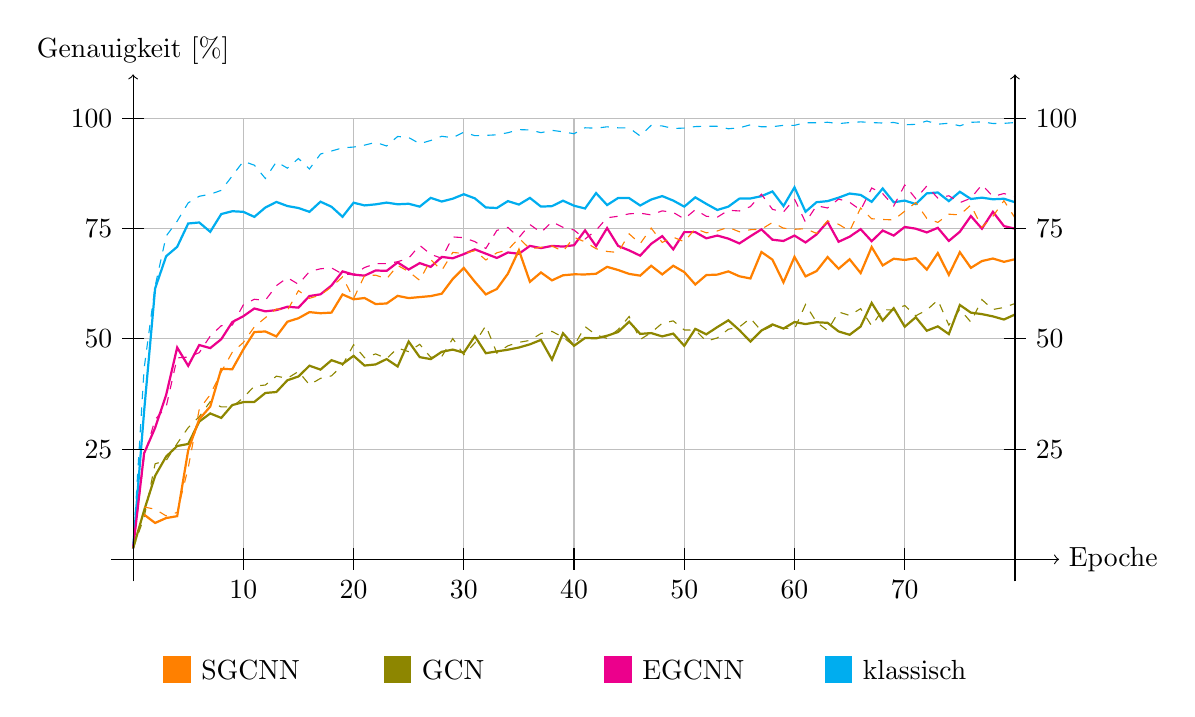
\begin{tikzpicture}[scale=1.4]
  \draw[color=lightgray] (0, 0) grid (8, 4);

  \tikzstyle{klassisch}=[color=cyan]
  \tikzstyle{egcnn}=[color=magenta]
  \tikzstyle{sgcnn}=[color=orange]
  \tikzstyle{gcn}=[color=olive]
  \tikzstyle{fillklassisch}=[fill=cyan]
  \tikzstyle{fillegcnn}=[fill=magenta]
  \tikzstyle{fillsgcnn}=[fill=orange]
  \tikzstyle{fillgcn}=[fill=olive]

  \draw[klassisch, dashed] (0, 0.1) -- (0.1, 1.7312) -- (0.2, 2.4792) -- (0.3, 2.933) -- (0.4, 3.0682) -- (0.5, 3.2344) -- (0.6, 3.2938) -- (0.7, 3.3125) -- (0.8, 3.3477) -- (0.9, 3.4792) -- (1.0, 3.6111) -- (1.1, 3.5759) -- (1.2, 3.4554) -- (1.3, 3.6066) -- (1.4, 3.5491) -- (1.5, 3.6364) -- (1.6, 3.5417) -- (1.7, 3.6771) -- (1.8, 3.7045) -- (1.9, 3.733) -- (2.0, 3.7404) -- (2.1, 3.7578) -- (2.2, 3.7831) -- (2.3, 3.75) -- (2.4, 3.8365) -- (2.5, 3.8269) -- (2.6, 3.7708) -- (2.7, 3.8) -- (2.8, 3.8382) -- (2.9, 3.825) -- (3.0, 3.875) -- (3.1, 3.8438) -- (3.2, 3.8462) -- (3.3, 3.8516) -- (3.4, 3.8705) -- (3.5, 3.8984) -- (3.6, 3.8958) -- (3.7, 3.8708) -- (3.8, 3.892) -- (3.9, 3.8787) -- (4.0, 3.8611) -- (4.1, 3.9152) -- (4.2, 3.9115) -- (4.3, 3.9241) -- (4.4, 3.9148) -- (4.5, 3.9141) -- (4.6, 3.8409) -- (4.7, 3.9375) -- (4.8, 3.9318) -- (4.9, 3.9087) -- (5.0, 3.9125) -- (5.1, 3.9261) -- (5.2, 3.9292) -- (5.3, 3.9286) -- (5.4, 3.9062) -- (5.5, 3.9148) -- (5.6, 3.9423) -- (5.7, 3.9241) -- (5.8, 3.925) -- (5.9, 3.9375) -- (6.0, 3.9375) -- (6.1, 3.9615) -- (6.2, 3.9605) -- (6.3, 3.9653) -- (6.4, 3.9531) -- (6.5, 3.9625) -- (6.6, 3.9688) -- (6.7, 3.9625) -- (6.8, 3.9583) -- (6.9, 3.9635) -- (7.0, 3.9423) -- (7.1, 3.9464) -- (7.2, 3.9766) -- (7.3, 3.9479) -- (7.4, 3.9562) -- (7.5, 3.933) -- (7.6, 3.9648) -- (7.7, 3.9688) -- (7.8, 3.9542) -- (7.9, 3.9554) -- (8.0, 3.9625);

  \draw[klassisch, thick] (0, 0.1) -- (0.1, 1.3438) -- (0.2, 2.4583) -- (0.3, 2.75) -- (0.4, 2.8352) -- (0.5, 3.0469) -- (0.6, 3.0562) -- (0.7, 2.9716) -- (0.8, 3.1328) -- (0.9, 3.1583) -- (1.0, 3.1528) -- (1.1, 3.1071) -- (1.2, 3.192) -- (1.3, 3.2426) -- (1.4, 3.2054) -- (1.5, 3.1875) -- (1.6, 3.1528) -- (1.7, 3.2448) -- (1.8, 3.1989) -- (1.9, 3.108) -- (2.0, 3.2356) -- (2.1, 3.2109) -- (2.2, 3.2206) -- (2.3, 3.2366) -- (2.4, 3.2212) -- (2.5, 3.226) -- (2.6, 3.2) -- (2.7, 3.2792) -- (2.8, 3.2463) -- (2.9, 3.2719) -- (3.0, 3.3125) -- (3.1, 3.275) -- (3.2, 3.1923) -- (3.3, 3.1875) -- (3.4, 3.25) -- (3.5, 3.2188) -- (3.6, 3.2792) -- (3.7, 3.2) -- (3.8, 3.2045) -- (3.9, 3.2537) -- (4.0, 3.2083) -- (4.1, 3.183) -- (4.2, 3.3229) -- (4.3, 3.2143) -- (4.4, 3.2784) -- (4.5, 3.2773) -- (4.6, 3.2102) -- (4.7, 3.2644) -- (4.8, 3.2955) -- (4.9, 3.2548) -- (5.0, 3.2) -- (5.1, 3.2841) -- (5.2, 3.225) -- (5.3, 3.1696) -- (5.4, 3.2) -- (5.5, 3.2727) -- (5.6, 3.274) -- (5.7, 3.2946) -- (5.8, 3.3375) -- (5.9, 3.2054) -- (6.0, 3.375) -- (6.1, 3.1538) -- (6.2, 3.2401) -- (6.3, 3.25) -- (6.4, 3.2812) -- (6.5, 3.3188) -- (6.6, 3.3062) -- (6.7, 3.2437) -- (6.8, 3.3646) -- (6.9, 3.2396) -- (7.0, 3.2548) -- (7.1, 3.2232) -- (7.2, 3.3203) -- (7.3, 3.3281) -- (7.4, 3.25) -- (7.5, 3.3348) -- (7.6, 3.2695) -- (7.7, 3.2812) -- (7.8, 3.2667) -- (7.9, 3.2715) -- (8.0, 3.2396);

  \draw[egcnn, thick] (0, 0.1) -- (0.1, 0.9625) -- (0.2, 1.1938) -- (0.3, 1.4922) -- (0.4, 1.9219) -- (0.5, 1.7557) -- (0.6, 1.9444) -- (0.7, 1.9167) -- (0.8, 1.9973) -- (0.9, 2.1528) -- (1.0, 2.2059) -- (1.1, 2.276) -- (1.2, 2.25) -- (1.3, 2.2614) -- (1.4, 2.2917) -- (1.5, 2.2837) -- (1.6, 2.3889) -- (1.7, 2.4044) -- (1.8, 2.4844) -- (1.9, 2.6125) -- (2.0, 2.5833) -- (2.1, 2.5739) -- (2.2, 2.6208) -- (2.3, 2.6172) -- (2.4, 2.6938) -- (2.5, 2.6295) -- (2.6, 2.6875) -- (2.7, 2.6534) -- (2.8, 2.7437) -- (2.9, 2.7313) -- (3.0, 2.7692) -- (3.1, 2.8125) -- (3.2, 2.7734) -- (3.3, 2.7344) -- (3.4, 2.7841) -- (3.5, 2.7723) -- (3.6, 2.8438) -- (3.7, 2.8239) -- (3.8, 2.8438) -- (3.9, 2.8375) -- (4.0, 2.85) -- (4.1, 2.9844) -- (4.2, 2.8413) -- (4.3, 3.0052) -- (4.4, 2.8438) -- (4.5, 2.8029) -- (4.6, 2.7552) -- (4.7, 2.8625) -- (4.8, 2.9323) -- (4.9, 2.8125) -- (5.0, 2.9688) -- (5.1, 2.9688) -- (5.2, 2.9125) -- (5.3, 2.9375) -- (5.4, 2.9097) -- (5.5, 2.8661) -- (5.6, 2.9312) -- (5.7, 2.9937) -- (5.8, 2.9) -- (5.9, 2.8884) -- (6.0, 2.9375) -- (6.1, 2.875) -- (6.2, 2.9479) -- (6.3, 3.0625) -- (6.4, 2.8813) -- (6.5, 2.9271) -- (6.6, 2.9952) -- (6.7, 2.8864) -- (6.8, 2.983) -- (6.9, 2.9375) -- (7.0, 3.0156) -- (7.1, 3.0) -- (7.2, 2.9659) -- (7.3, 3.0078) -- (7.4, 2.8889) -- (7.5, 2.9722) -- (7.6, 3.1146) -- (7.7, 3.0) -- (7.8, 3.1528) -- (7.9, 3.0234) -- (8.0, 3.0);

  \draw[egcnn, dashed] (0, 0.1) -- (0.1, 0.9313) -- (0.2, 1.2688) -- (0.3, 1.3828) -- (0.4, 1.8281) -- (0.5, 1.8352) -- (0.6, 1.875) -- (0.7, 2.026) -- (0.8, 2.1196) -- (0.9, 2.125) -- (1.0, 2.3088) -- (1.1, 2.3594) -- (1.2, 2.35) -- (1.3, 2.483) -- (1.4, 2.5556) -- (1.5, 2.4952) -- (1.6, 2.6111) -- (1.7, 2.636) -- (1.8, 2.6445) -- (1.9, 2.5875) -- (2.0, 2.5833) -- (2.1, 2.6477) -- (2.2, 2.6833) -- (2.3, 2.6836) -- (2.4, 2.7) -- (2.5, 2.7321) -- (2.6, 2.849) -- (2.7, 2.767) -- (2.8, 2.7313) -- (2.9, 2.925) -- (3.0, 2.9183) -- (3.1, 2.8828) -- (3.2, 2.8203) -- (3.3, 2.9844) -- (3.4, 3.0114) -- (3.5, 2.9196) -- (3.6, 3.0375) -- (3.7, 2.9659) -- (3.8, 3.0625) -- (3.9, 3.0125) -- (4.0, 2.9875) -- (4.1, 2.9062) -- (4.2, 2.9856) -- (4.3, 3.099) -- (4.4, 3.1125) -- (4.5, 3.1346) -- (4.6, 3.1406) -- (4.7, 3.125) -- (4.8, 3.1615) -- (4.9, 3.1477) -- (5.0, 3.0885) -- (5.1, 3.1719) -- (5.2, 3.1125) -- (5.3, 3.1042) -- (5.4, 3.1667) -- (5.5, 3.1607) -- (5.6, 3.2) -- (5.7, 3.3125) -- (5.8, 3.175) -- (5.9, 3.1518) -- (6.0, 3.2692) -- (6.1, 3.0583) -- (6.2, 3.2083) -- (6.3, 3.1875) -- (6.4, 3.2687) -- (6.5, 3.2396) -- (6.6, 3.1683) -- (6.7, 3.3693) -- (6.8, 3.3182) -- (6.9, 3.2062) -- (7.0, 3.3958) -- (7.1, 3.2723) -- (7.2, 3.3864) -- (7.3, 3.2773) -- (7.4, 3.2986) -- (7.5, 3.2361) -- (7.6, 3.276) -- (7.7, 3.399) -- (7.8, 3.2917) -- (7.9, 3.3188) -- (8.0, 3.2891);

  \draw[gcn, dashed] (0, 0.1) -- (0.1, 0.3812) -- (0.2, 0.8672) -- (0.3, 0.8973) -- (0.4, 1.0511) -- (0.5, 1.1953) -- (0.6, 1.2937) -- (0.7, 1.4318) -- (0.8, 1.3833) -- (0.9, 1.3833) -- (1.0, 1.4669) -- (1.1, 1.5714) -- (1.2, 1.5817) -- (1.3, 1.6618) -- (1.4, 1.6429) -- (1.5, 1.7045) -- (1.6, 1.5833) -- (1.7, 1.642) -- (1.8, 1.6648) -- (1.9, 1.7614) -- (2.0, 1.9471) -- (2.1, 1.8292) -- (2.2, 1.864) -- (2.3, 1.8214) -- (2.4, 1.9167) -- (2.5, 1.8846) -- (2.6, 1.9509) -- (2.7, 1.8333) -- (2.8, 1.8398) -- (2.9, 2.0031) -- (3.0, 1.8562) -- (3.1, 1.9625) -- (3.2, 2.1202) -- (3.3, 1.8711) -- (3.4, 1.9375) -- (3.5, 1.9688) -- (3.6, 1.9866) -- (3.7, 2.0491) -- (3.8, 2.0682) -- (3.9, 2.0147) -- (4.0, 1.9375) -- (4.1, 2.1116) -- (4.2, 2.0365) -- (4.3, 2.0048) -- (4.4, 2.0852) -- (4.5, 2.2031) -- (4.6, 1.9943) -- (4.7, 2.0577) -- (4.8, 2.142) -- (4.9, 2.1635) -- (5.0, 2.0812) -- (5.1, 2.0795) -- (5.2, 1.9792) -- (5.3, 2.0089) -- (5.4, 2.0875) -- (5.5, 2.108) -- (5.6, 2.1875) -- (5.7, 2.0714) -- (5.8, 2.1187) -- (5.9, 2.0982) -- (6.0, 2.0909) -- (6.1, 2.3125) -- (6.2, 2.1513) -- (6.3, 2.0764) -- (6.4, 2.2448) -- (6.5, 2.2125) -- (6.6, 2.275) -- (6.7, 2.1181) -- (6.8, 2.2656) -- (6.9, 2.2614) -- (7.0, 2.3029) -- (7.1, 2.2098) -- (7.2, 2.2617) -- (7.3, 2.3523) -- (7.4, 2.125) -- (7.5, 2.2692) -- (7.6, 2.1523) -- (7.7, 2.3563) -- (7.8, 2.2667) -- (7.9, 2.2852) -- (8.0, 2.3210);

  \draw[gcn, thick] (0, 0.1) -- (0.1, 0.4437) -- (0.2, 0.7578) -- (0.3, 0.933) -- (0.4, 1.0284) -- (0.5, 1.0469) -- (0.6, 1.25) -- (0.7, 1.3239) -- (0.8, 1.2833) -- (0.9, 1.4) -- (1.0, 1.4265) -- (1.1, 1.4286) -- (1.2, 1.5096) -- (1.3, 1.5184) -- (1.4, 1.625) -- (1.5, 1.6591) -- (1.6, 1.7569) -- (1.7, 1.7216) -- (1.8, 1.8068) -- (1.9, 1.7727) -- (2.0, 1.8462) -- (2.1, 1.7583) -- (2.2, 1.7684) -- (2.3, 1.817) -- (2.4, 1.75) -- (2.5, 1.976) -- (2.6, 1.8348) -- (2.7, 1.8167) -- (2.8, 1.8828) -- (2.9, 1.9031) -- (3.0, 1.875) -- (3.1, 2.025) -- (3.2, 1.8702) -- (3.3, 1.8867) -- (3.4, 1.9018) -- (3.5, 1.9219) -- (3.6, 1.9509) -- (3.7, 1.9911) -- (3.8, 1.8125) -- (3.9, 2.0515) -- (4.0, 1.9375) -- (4.1, 2.0089) -- (4.2, 2.0052) -- (4.3, 2.0288) -- (4.4, 2.0625) -- (4.5, 2.1562) -- (4.6, 2.0455) -- (4.7, 2.0529) -- (4.8, 2.0227) -- (4.9, 2.0481) -- (5.0, 1.9375) -- (5.1, 2.0909) -- (5.2, 2.0417) -- (5.3, 2.1071) -- (5.4, 2.1688) -- (5.5, 2.0795) -- (5.6, 1.976) -- (5.7, 2.0759) -- (5.8, 2.1313) -- (5.9, 2.0938) -- (6.0, 2.1534) -- (6.1, 2.1346) -- (6.2, 2.1513) -- (6.3, 2.1458) -- (6.4, 2.0677) -- (6.5, 2.0375) -- (6.6, 2.1125) -- (6.7, 2.3264) -- (6.8, 2.1667) -- (6.9, 2.2784) -- (7.0, 2.1106) -- (7.1, 2.1964) -- (7.2, 2.0742) -- (7.3, 2.1136) -- (7.4, 2.0438) -- (7.5, 2.3077) -- (7.6, 2.2383) -- (7.7, 2.225) -- (7.8, 2.2042) -- (7.9, 2.1758) -- (8.0, 2.2214);

  \draw[sgcnn, thick] (0.1, 0.4062) -- (0.2, 0.3304) -- (0.3, 0.375) -- (0.4, 0.392) -- (0.5, 0.9911) -- (0.6, 1.2708) -- (0.7, 1.3864) -- (0.8, 1.7277) -- (0.9, 1.725) -- (1.0, 1.9044) -- (1.1, 2.0625) -- (1.2, 2.0673) -- (1.3, 2.0223) -- (1.4, 2.1562) -- (1.5, 2.1875) -- (1.6, 2.2431) -- (1.7, 2.233) -- (1.8, 2.2386) -- (1.9, 2.4034) -- (2.0, 2.3594) -- (2.1, 2.3708) -- (2.2, 2.3164) -- (2.3, 2.3214) -- (2.4, 2.3906) -- (2.5, 2.3702) -- (2.6, 2.3795) -- (2.7, 2.3884) -- (2.8, 2.4102) -- (2.9, 2.5438) -- (3.0, 2.6437) -- (3.1, 2.5187) -- (3.2, 2.4038) -- (3.3, 2.4531) -- (3.4, 2.5913) -- (3.5, 2.8047) -- (3.6, 2.5179) -- (3.7, 2.6027) -- (3.8, 2.5312) -- (3.9, 2.5772) -- (4.0, 2.5859) -- (4.1, 2.5848) -- (4.2, 2.5909) -- (4.3, 2.6538) -- (4.4, 2.625) -- (4.5, 2.5898) -- (4.6, 2.5739) -- (4.7, 2.6635) -- (4.8, 2.5852) -- (4.9, 2.6635) -- (5.0, 2.6063) -- (5.1, 2.4937) -- (5.2, 2.5792) -- (5.3, 2.5833) -- (5.4, 2.6125) -- (5.5, 2.5682) -- (5.6, 2.5481) -- (5.7, 2.7885) -- (5.8, 2.7188) -- (5.9, 2.5134) -- (6.0, 2.7443) -- (6.1, 2.5673) -- (6.2, 2.6151) -- (6.3, 2.7422) -- (6.4, 2.6364) -- (6.5, 2.7222) -- (6.6, 2.5972) -- (6.7, 2.8333) -- (6.8, 2.6667) -- (6.9, 2.7273) -- (7.0, 2.7163) -- (7.1, 2.7321) -- (7.2, 2.6289) -- (7.3, 2.7784) -- (7.4, 2.5812) -- (7.5, 2.7865) -- (7.6, 2.6445) -- (7.7, 2.7062) -- (7.8, 2.7292) -- (7.9, 2.6992) -- (8.0, 2.7227);

  \draw[sgcnn, dashed] (0.1, 0.475) -- (0.2, 0.4554) -- (0.3, 0.3942) -- (0.4, 0.4261) -- (0.5, 0.8304) -- (0.6, 1.3611) -- (0.7, 1.4943) -- (0.8, 1.7009) -- (0.9, 1.8792) -- (1.0, 1.9669) -- (1.1, 2.1094) -- (1.2, 2.1923) -- (1.3, 2.2723) -- (1.4, 2.2589) -- (1.5, 2.4375) -- (1.6, 2.3681) -- (1.7, 2.3977) -- (1.8, 2.4716) -- (1.9, 2.5625) -- (2.0, 2.3646) -- (2.1, 2.575) -- (2.2, 2.5781) -- (2.3, 2.5446) -- (2.4, 2.6667) -- (2.5, 2.6106) -- (2.6, 2.5312) -- (2.7, 2.7188) -- (2.8, 2.6211) -- (2.9, 2.7844) -- (3.0, 2.775) -- (3.1, 2.8) -- (3.2, 2.7163) -- (3.3, 2.7812) -- (3.4, 2.8077) -- (3.5, 2.9141) -- (3.6, 2.817) -- (3.7, 2.8304) -- (3.8, 2.8438) -- (3.9, 2.7941) -- (4.0, 2.9219) -- (4.1, 2.8795) -- (4.2, 2.8182) -- (4.3, 2.7933) -- (4.4, 2.7841) -- (4.5, 2.9531) -- (4.6, 2.8636) -- (4.7, 3.0048) -- (4.8, 2.875) -- (4.9, 2.9231) -- (5.0, 2.8813) -- (5.1, 3.0) -- (5.2, 2.9625) -- (5.3, 2.9792) -- (5.4, 3.0125) -- (5.5, 2.9716) -- (5.6, 2.9904) -- (5.7, 2.9952) -- (5.8, 3.0562) -- (5.9, 3.0045) -- (6.0, 2.9943) -- (6.1, 3.0) -- (6.2, 2.9572) -- (6.3, 3.0703) -- (6.4, 3.0398) -- (6.5, 2.9792) -- (6.6, 3.1875) -- (6.7, 3.0903) -- (6.8, 3.0833) -- (6.9, 3.0795) -- (7.0, 3.1587) -- (7.1, 3.2366) -- (7.2, 3.0938) -- (7.3, 3.0568) -- (7.4, 3.1313) -- (7.5, 3.125) -- (7.6, 3.2148) -- (7.7, 3.0125) -- (7.8, 3.1125) -- (7.9, 3.2539) -- (8.0, 3.0977);


  \draw (0.1, 4) -- (-0.1, 4) node[left] {$100$};
  \draw (0.1, 3) -- (-0.1, 3) node[left] {$75$};
  \draw (0.1, 2) -- (-0.1, 2) node[left] {$50$};
  \draw (0.1, 1) -- (-0.1, 1) node[left] {$25$};

  \draw (7.9, 4) -- (8.1, 4) node[right] {$100$};
  \draw (7.9, 3) -- (8.1, 3) node[right] {$75$};
  \draw (7.9, 2) -- (8.1, 2) node[right] {$50$};
  \draw (7.9, 1) -- (8.1, 1) node[right] {$25$};

  \draw (1, 0.1) -- (1, -0.1)  node[below] {$10$};
  \draw (2, 0.1) -- (2, -0.1)  node[below] {$20$};
  \draw (3, 0.1) -- (3, -0.1)  node[below] {$30$};
  \draw (4, 0.1) -- (4, -0.1)  node[below] {$40$};
  \draw (5, 0.1) -- (5, -0.1)  node[below] {$50$};
  \draw (6, 0.1) -- (6, -0.1)  node[below] {$60$};
  \draw (7, 0.1) -- (7, -0.1)  node[below] {$70$};

  \draw[->] (-0.2, 0)    -- (8.4, 0)   node[right] {Epoche};
  \draw[->] (0,    -0.2) -- (0,   4.4) node[above] {Genauigkeit [\%]};
  \draw[->] (8,    -0.2) -- (8,   4.4);

  \tikzstyle{node}=[rectangle, minimum width=10pt, minimum height=10pt, inner sep=0pt]
  \node[node, fillsgcnn,     label=right:\gls{SGCNN}] (1) at (0.4, -1) {};
  \node[node, fillgcn,       label=right:\gls{GCN}]   (2) at (2.4, -1) {};
  \node[node, fillegcnn,     label=right:\gls{EGCNN}] (3) at (4.4, -1) {};
  \node[node, fillklassisch, label=right:klassisch]   (4) at (6.4, -1) {};

\end{tikzpicture}
\caption[\gls{Cifar}-10 Genauigkeitsverlauf über Quickshift]{Genauigkeitsverlauf eines Trainings auf dem \gls{Cifar}-10 Datensatz der spektralen Ansätze auf Graphen im zweidimensionalen euklidischen Raum, welche über Quickshift generiert wurden, sowie dem klassischen Ansatz auf Bildern.
Die gestrichelten Linien zeigen die Genauigkeiten des Trainingsdatensatzes in Abhängigkeit der Epochen, wohingegen die durchgezogenen Linien sich auf den Validierungsdatensatz beziehen.}
\label{fig:cifar_10_train}
\end{figure}


Postprocessing weitaus besser als preprocessing!

Mit drei mal Dropout kein Overfitting, trainiert allerdings langsam
Learning Rate Decay darf nicht zu krass sein

Durchschnittliche Faltungsdauer: 2.05s, Preprocessingdauer: 0.35s
Bei Batch-Size 64
Erstes Resultat mit Postprocessing:
Loss: 1.05440, acc: 0.63411

Zweiter Test:
Dropout nur noch 2 mal, nicht so starkes Learning Rate Decay
ist nun bei 70 \% nach 50k Steps
Dropout ist immer noch zu hart

Alle Faltungen wurden dabei mit einer Partitionsgröße von $8$ bei $K=0$ und $K=1$ implementiert, um ein \gls{CNN} mit einem $3 \times 3$ Filter zu simulieren.
Es erscheint jedoch vorstellbar die Filtergröße bei größerer lokaler Kontrollierbarkeit, \dhe{} $K > 1$, weiter zu reduzieren und die Gefahr des Overfittings damit aufgrund der kleineren Anzahl an Trainingsparametern einzuschränken.
